\section{Results}
\label{sec:results}

We organize results around five questions. Symbolic and Qwen conditions are never pooled.

\subsection{Are accuracy and consistency distinct?}

\paragraph{Corruption suite (smoke).} Gold predictions attain Acc $=$ BCR $=$ ConsAcc $=$ 1. Controlled corruptions separate the metrics (Table~\ref{tab:corruption}). High Acc with BCR~$=$~0 and low Acc with BCR~$=$~1 both occur. This supports that $\Phi$ is not redundant with Acc.

\begin{table}[t]
\centering
\caption{Corruption-suite validation (smoke; frozen).}
\label{tab:corruption}
\begin{tabular}{lrrr}
\toprule
Corruption & Acc & BCR & $\Gapq$ \\
\midrule
high\_acc\_inconsistent & 0.849 & 0.000 & 0.849 \\
wrong\_provenance & 0.849 & 0.000 & 0.849 \\
consistent\_wrong\_world & 0.394 & 1.000 & $-$0.606 \\
transition\_inconsistency & 0.939 & 0.600 & 0.339 \\
\bottomrule
\end{tabular}
\end{table}

\subsection{Does the distinction persist at scale?}

\paragraph{Symbolic scaled (102 worlds).} Retrieval baselines show large Acc--BCR gaps (Table~\ref{tab:symbolic}; Figure~\ref{fig:accbcr}, left). B4 retains high Acc while BCR remains materially lower ($\Gapq=0.338$). The Acc--consistency distinction survives scaling under the deterministic reader. World-level bootstrap CIs are reported in the frozen statistical analysis artefacts.

\begin{table}[t]
\centering
\caption{Symbolic scaled results (102 worlds; frozen). Acc, BCR, CSR rounded half-up to three decimals from frozen point estimates.}
\label{tab:symbolic}
\begin{tabular}{lrrrr}
\toprule
System & Acc & BCR & $\Gapq$ & mean CSR \\
\midrule
B3 recency-$k8$ & 0.567 & 0.063 & 0.504 & 0.507 \\
B4 BM25-$k8$ & 0.929 & 0.591 & 0.338 & 0.881 \\
B1 compact (cap150) & 1.000 & 1.000 & 0.000 & 1.000 \\
H0 LTKM (cap150, ret8) & 0.976 & 0.844 & 0.132 & 0.973 \\
\bottomrule
\end{tabular}
\end{table}

\begin{figure}[t]
\centering
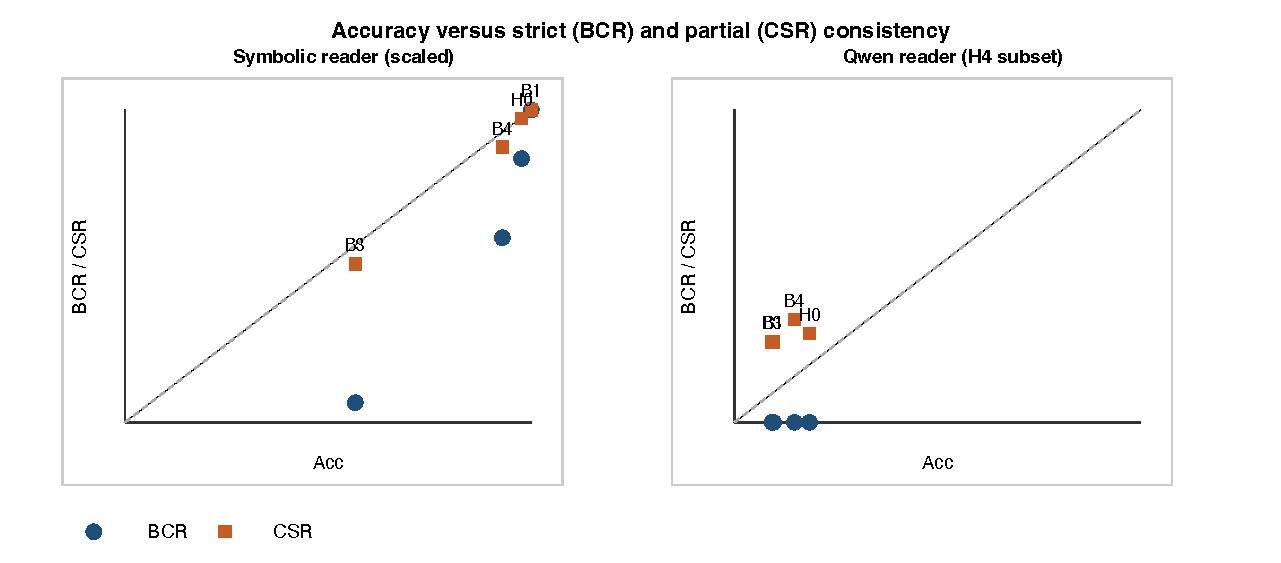
\includegraphics[width=\linewidth]{figures/fig3-acc-vs-bcr-csr.pdf}
\caption{Acc versus BCR and CSR under symbolic and Qwen readers.}
\label{fig:accbcr}
\end{figure}

\subsection{Which systems show the largest gaps?}

Under the symbolic reader, \textbf{recency retrieval} exhibits the largest $\Gapq$ among the headline retrieval points (0.504). \textbf{BM25} narrows but does not close the gap. \textbf{Compact flat at capacity 150} saturates Acc and BCR in this generator regime (fairness caveat: padding eviction can preserve focal lifecycle evidence; Section~\ref{sec:systems}). \textbf{H0 at cap150/ret8} achieves high Acc and high BCR/CSR, but does \textbf{not} beat compact flat on BCR ($\Delta$BCR vs compact $=$ $-$0.156 at this point; matched lift vs compact fails the frozen gate). H0 does beat matched \textbf{recency} flat on BCR in the frozen capacity study; that is a matched-baseline comparison, not a claim of architectural superiority over all flat stores.

Selective ablations (archive, temporal-validity, graph, conflict) produce family-level Acc drops in the frozen ablation table; they are diagnostic of component--family links under the symbolic reader, not evidence that a multi-component store is necessary. Stratified Acc/BCR by difficulty and tier are shown in Figure~\ref{fig:difficulty} (Appendix~\ref{app:extrafigs}).

\subsection{What happens under the Qwen reader?}

\paragraph{H4 subset; frozen Qwen Option A.} All four systems have \textbf{BCR~$=$~0}. Acc remains ordered (Table~\ref{tab:qwen}; Figure~\ref{fig:accbcr}, right). Because the constraint suite is satisfiable for gold/oracle predictions and yields non-trivial BCR on the deterministic symbolic reader (Section~\ref{sec:benchmark} smoke confirmation and Section~\ref{sec:results} symbolic results), the Qwen BCR floor reflects difficulty in producing jointly constraint-satisfying answers under this frozen reader/parsing pipeline, not an intrinsically inconsistent constraint definition.

\begin{table}[t]
\centering
\caption{Qwen H4 Option A results (18 worlds, 192 bundles; frozen). Values rounded half-up to three decimals. All PConsAcc grid cells at $(\tau,\tau_c)\in\{0.5,0.8\}\times\{0.8,0.9\}$ are 0.}
\label{tab:qwen}
\begin{tabular}{lrrrrr}
\toprule
System & Acc & BCR & mean CSR & Abs & Mal \\
\midrule
B1 compact & 0.096 & 0.000 & 0.258 & 0.728 & 0.007 \\
B3 recency-$k8$ & 0.093 & 0.000 & 0.258 & 0.728 & 0.007 \\
B4 BM25-$k8$ & 0.148 & 0.000 & 0.329 & 0.579 & 0.001 \\
H0 LTKM & 0.185 & 0.000 & 0.284 & 0.483 & 0.029 \\
\bottomrule
\end{tabular}
\end{table}

\paragraph{Reading.}
\begin{itemize}[leftmargin=*,itemsep=1pt]
\item In this Qwen setting, H0 has the \textbf{highest Acc} and lower abstention than flats/recency.
\item B4 has the \textbf{highest CSR}.
\item H0's CSR is above B1/B3 ($+$0.026) but \textbf{below B4 ($-$0.045)}.
\item \textbf{No architecture consistency advantage is supported} under Qwen: BCR ties at 0; CSR does not rank H0 highest.
\item Acc gains must not be converted into consistency claims.
\end{itemize}

\subsection{Does CSR provide resolution when BCR floors?}

Yes, within limits. With BCR~$=$~0 for all Qwen systems, mean CSR still separates B4 (0.329) from B1/B3 (0.258) and H0 (0.284). Mean violations per bundle remain high ($\approx$3.3--3.6). Acc--CSR Pearson correlation is positive for B1/B3/B4 ($\approx$0.30--0.43) but near zero/slightly negative for H0 ($-$0.04), consistent with H0 answering more questions without proportional joint constraint satisfaction.

\paragraph{Conclusion of Section~\ref{sec:results}.} Acc and consistency are empirically distinct; the distinction persists symbolically at scale; under Qwen, strict BCR floors while CSR remains weakly diagnostic; the structured reference H0 is not supported as a consistency winner under Qwen.
